
%%%%%%%%%%%%%%%%%%%%%%%%%%%%%%%%%%%%%%%%%%%%%%%%%%%%%%%%%%%%%%%%%%%%%%%%%%%%%%%%%%%%%%%
%%%%%%%%%%%%%%%%%%%%%%%%%%%%%%%%%%%%%%%%%%%%%%%%%%%%%%%%%%%%%%%%%%%%%%%%%%%%%%%%%%%%%%%
% 
% This top part of the document is called the 'preamble'.  Modify it with caution!
%
% The real document starts below where it says 'The main document starts here'.

\documentclass[12pt]{article}

\usepackage{amssymb,amsmath,amsthm}
\usepackage[top=1in, bottom=1in, left=1.25in, right=1.25in]{geometry}
\usepackage{fancyhdr}
\usepackage{enumerate}
\usepackage{listings}
\usepackage{graphicx}
\usepackage{float}

\usepackage{mwe}
\usepackage{caption}
\usepackage{subcaption}
% Comment the following line to use TeX's default font of Computer Modern.
\usepackage{times,txfonts}



\makeatletter
\renewcommand*\env@matrix[1][*\c@MaxMatrixCols c]{%
  \hskip -\arraycolsep
  \let\@ifnextchar\new@ifnextchar
  \array{#1}}
\makeatother

\newtheoremstyle{homework}% name of the style to be used
  {18pt}% measure of space to leave above the theorem. E.g.: 3pt
  {12pt}% measure of space to leave below the theorem. E.g.: 3pt
  {}% name of font to use in the body of the theorem
  {}% measure of space to indent
  {\bfseries}% name of head font
  {:}% punctuation between head and body
  {2ex}% space after theorem head; " " = normal interword space
  {}% Manually specify head
\theoremstyle{homework} 

% Set up an Exercise environment and a Solution label.
\newtheorem*{exercisecore}{Exercise \@currentlabel}
\newenvironment{exercise}[1]
{\def\@currentlabel{#1}\exercisecore}
{\endexercisecore}

\newcommand{\localhead}[1]{\par\smallskip\noindent\textbf{#1}\nobreak\\}%
\newcommand\solution{\localhead{Solution:}}

%%%%%%%%%%%%%%%%%%%%%%%%%%%%%%%%%%%%%%%%%%%%%%%%%%%%%%%%%%%%%%%%%%%%%%%%
%
% Stuff for getting the name/document date/title across the header
\makeatletter
\RequirePackage{fancyhdr}
\pagestyle{fancy}
\fancyfoot[C]{\ifnum \value{page} > 1\relax\thepage\fi}
\fancyhead[L]{\ifx\@doclabel\@empty\else\@doclabel\fi}
\fancyhead[C]{\ifx\@docdate\@empty\else\@docdate\fi}
\fancyhead[R]{\ifx\@docauthor\@empty\else\@docauthor\fi}
\headheight 15pt

\def\doclabel#1{\gdef\@doclabel{#1}}
\doclabel{Use {\tt\textbackslash doclabel\{MY LABEL\}}.}
\def\docdate#1{\gdef\@docdate{#1}}
\docdate{Use {\tt\textbackslash docdate\{MY DATE\}}.}
\def\docauthor#1{\gdef\@docauthor{#1}}
\docauthor{Use {\tt\textbackslash docauthor\{MY NAME\}}.}
\makeatother

% Shortcuts for blackboard bold number sets (reals, integers, etc.)
\newcommand{\Reals}{\ensuremath{\mathbb R}}
\newcommand{\Nats}{\ensuremath{\mathbb N}}
\newcommand{\Ints}{\ensuremath{\mathbb Z}}
\newcommand{\Rats}{\ensuremath{\mathbb Q}}
\newcommand{\Cplx}{\ensuremath{\mathbb C}}
%% Some equivalents that some people may prefer.
\let\RR\Reals
\let\NN\Nats
\let\II\Ints
\let\CC\Cplx
%%%%%%%%%%%%%%%%%%%%%%%%%%%%%%%%%%%%%%%%%%%%%%%%%%%%%%%%%%%%%%%%%%%%%%%%%%%%%%%%%%%%%%%
%%%%%%%%%%%%%%%%%%%%%%%%%%%%%%%%%%%%%%%%%%%%%%%%%%%%%%%%%%%%%%%%%%%%%%%%%%%%%%%%%%%%%%%
% 
% The main document start here.

% The following commands set up the material that appears in the header.
\doclabel{Stat 461: Homework 1}
\docauthor{Stefano Fochesatto}
\docdate{\today}

\begin{document}

\begin{exercise}{1} What is a row vector, what is a column vector?\\
  \solution row and column vectors are simply vectors, but in the context of matrices. A matrix has 
  two spaces/dimensions, the row space and column space. We can think of row and column vectors as matrices 
  with a single dimension, i.e a 1xn matrix would be a column vector and a nx1 matrix would be a row vector. 
\end{exercise}
\vspace{1in}

\begin{exercise}{2} The following is an rxc matrix. What are r and c, as well as the matrices transpose.
  \begin{equation*}
    A = \begin{bmatrix}
      1&2&3&4 \\
      2&1&2&1 
    \end{bmatrix}
  \end{equation*}
  \solution A is a 2x4 matrix, where $r = 2$ and $c = 4$, The following is the transpose, 
  \begin{equation*}
    A^T = \begin{bmatrix}
      1 & 2\\
      2 & 1\\
      3 & 2\\
      4 & 1
    \end{bmatrix}
  \end{equation*}
\end{exercise}
\vspace{1in}

\begin{exercise}{3} Give an example of an identity matrix and an example of a diagonal matrix.\\
  \solution The identity matrix is a diagonal matrix with all ones on the diagonal. The following is the 
  3x3 identity matrix, 
  \begin{equation*}
    I_{3x3} = \begin{bmatrix}
      1 &0 &0 \\
      0 &1 &0 \\
      0 &0 &1
    \end{bmatrix}
  \end{equation*}
  Identity matrices are a subset of diagonal matrices. The following is an example of diagonal matrix, 
  \begin{equation*}
    A = \begin{bmatrix}
      1 &0 &0 \\
      0 &2 &0 \\
      0 &0 &3
    \end{bmatrix}
  \end{equation*}
\end{exercise}
\vspace{1in}



\begin{exercise}{4} Is the following a symmetric matrix? why?\\
  \begin{equation*}
    A = 
    \begin{bmatrix}
      2 &3 &5 \\
      3 &4 &6 \\
      5 &6 &100
    \end{bmatrix}
  \end{equation*}
  \solution A is a symmetric matrix, since it has the property that $A = A^T$.
\end{exercise}
\vspace{1in}



\begin{exercise}{5} Consider the following matrices, 
  \begin{figure}[H]
    \begin{center}
    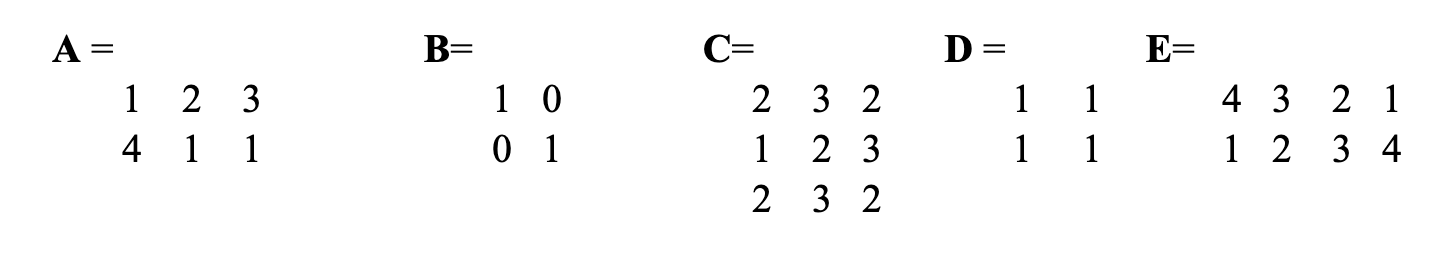
\includegraphics[width = .75\textwidth]{matrices.png}
    \end{center}
  \end{figure} 
  \begin{enumerate}
    \item[a.] Is $A + B$ undefined?\\
    \solution Matrix addition is done entrywise. Note $A$ is a 2x3 matrix and $B$ is 2x2 so this operations would be undefined.  
    \vspace{.15in}

    \item[b.] Is $AB$ undefined?\\
    \solution Matrix multiplication requires the inner dimensions to be equal. Note $A$ is a 2x3 matrix and $B$ is 2x2, since $3 \neq 2$ this operation would be undefined. 
    \vspace{.15in}
    

    \item[c.] Is $BA$ undefined?\\
    \solution The inner dimensions do match, so $BA$ is well defined. 
    \vspace{.15in}


    \item[d.] Is $E'D$ undefined?\\
    \solution Note that $E'$ is a 4x2 matrix and $D$ is a 2x2 matrix. This operation is well defined.  
    \vspace{.15in}


    \item[e.] Is $3E$ undefined?\\
    \solution $3E$ is well defined, we just multiply every term in $E$ by 3.   
  \end{enumerate}
\end{exercise}
\vspace{1in}



\begin{exercise}{6} Find the inverse of the following matrix, then compute $G^{-1}G$
  \begin{equation*}
    G = 
    \begin{bmatrix}
      1 & 2\\
      2 & 1
    \end{bmatrix}
    \end{equation*}
    \solution There is a formula for computing the inverse of a 2x2 matrix, which gives the following, 
    \begin{equation*}
      G^{-1} = 
      -\dfrac{1}{3}
      \begin{bmatrix}
        1 & -2\\
        -2 & 1
      \end{bmatrix}
    \end{equation*}
    Finally we know that the product of a matrix and its inverse is simply the identity. For this case we get $G^{-1}G = I_{2x2}$. 
\end{exercise}
\vspace{1in}



\begin{exercise}{7} Consider the following matrix, 
  \begin{equation*}
    Q = 
    \begin{bmatrix}
      4 &1 &1 \\ 
      1 &4 &1 \\ 
      1 &1 &4 
    \end{bmatrix}
  \end{equation*}
  Is $e = [ 1 1 1 ]'$ and eigenvector? If so show that it's eigenvalue is 6. 
  \solution We can check this by computing $Qe$. Doing so we get,
  \begin{equation*}
    \begin{bmatrix}
      4 &1 &1 \\ 
      1 &4 &1 \\ 
      1 &1 &4 
    \end{bmatrix}
    \begin{bmatrix}
      1\\ 
      1\\ 
      1 
    \end{bmatrix}
    =
    \begin{bmatrix}
      6\\ 
      6\\ 
      6 
    \end{bmatrix}
    =
    6
    \begin{bmatrix}
      1\\ 
      1\\ 
      1 
    \end{bmatrix}
  \end{equation*}
\end{exercise}
\vspace{1in}


\begin{exercise}{8} 
  \begin{enumerate}
    \item[a.] What is a p-value? If you knew a test had a p-value of .01 and it was performed at the $\alpha = .05$ significance level, 
    would you reject the null hypothesis?\\
    \solution The p-value is the probability of obtaining the test statistic under the assumption of the null hypothesis. In the situation described above we would reject the 
    null hypothesis since p-value is smaller than the significance level. The probability of attaining the test statistics is under the $\alpha = .05$ significance level is essentially zero. 
    \vspace{.15in}
    
    \item[b.] What does the significance level of a test tell you?\\
    \solution  The significance level of a test is the probability of rejecting the null hypothesis when it is true.
    \vspace{.15in}

    \item[c.] What is the difference between a parameter and a statistic?\\
    \solution A parameter describes an entire population, a statistic descirbes a sample of the population.
    \vspace{.15in}

    \item[d.] If you create a 95\% confidence interval for a parameter what does that tell you?\\
    \solution 95\% percent of all samples taken to estimate the parameter will give a value inside the interval.  

  \end{enumerate}
  
\end{exercise}



















\end{document}


















